\documentclass[twoside,a4paper]{refart}
\usepackage{makeidx}
\usepackage{ifthen}
\usepackage{datetime}
\usepackage{listings}
\usepackage{amsmath}
\usepackage{amssymb}
\usepackage{graphicx}
\usepackage{multirow}
\usepackage{caption}
\usepackage{url}
\usepackage{algorithm}
\usepackage{xtab,booktabs}
\usepackage{tabularx}
\usepackage[noend]{algpseudocode}
\renewcommand{\algorithmicensure}{\textbf{Output:}}
      
\def\bs{\char'134 } % backslash in \tt font.
\newcommand{\ie}{i.\,e.,}
\newcommand{\eg}{e.\,g..}
\DeclareRobustCommand\cs[1]{\texttt{\char`\\#1}}

\title{Stuffed Version 2.0}
\author{R. J. Lyon \thanks{Email: robert.lyon@postgrad.manchester.ac.uk , Web: \protect\url{www.scienceguyrob.com} .}\\
School of Computer Science \& \\
Jodrell Bank Centre for Astrophysics\\
University of Manchester\\
Kilburn Building\\
Oxford Road\\
Manchester M13 9PL\\
\date{\today}  
}

\date{}
\emergencystretch1em  %

\pagestyle{myfootings}
\markboth{Stuffed Version 2.0}%
         {Stuffed Version 2.0}

\makeindex 

\setcounter{tocdepth}{2}

\begin{document}

\maketitle

\begin{abstract}
The \textsc{stuffed} framework is a collection of Java files, which wrap around the WEKA and MOA frameworks.
The main goal of \textsc{stuffed} is to make it easier to perform experiments with unlabelled and partially-labelled \textit{imbalanced} data streams. Testing classifiers on such data streams is currently difficult to do within MOA and WEKA.\\

This API supplements MOA and WEKA functionality in a number of ways. It uses a custom sampling procedure to create data streams with varying proportions of labelled data, and varying levels of class imbalance. The API also enables the evaluation of classifiers on unlabelled data, thorough the use of custom meta data files, that allow true class labels to be retrieved during prediction evaluation. The API was developed specifically to enable the experiments described in \cite{Lyon:2013:jk,Lyon:2014:jk}.
\end{abstract}
\newpage

\tableofcontents

\newpage


%%%%%%%%%%%%%%%%%%%%%%%%%%%%%%%%%%%%%%%%%%%%%%%%%%%%%%%%%%%%%%%%%%%%

\section{Acknowledgements}
Thank you to the team responsible for developing MOA and WEKA. 

Development work was supported by grant EP/I028099/1 for the University of Manchester Centre for Doctoral Training in Computer Science, from the UK Engineering and Physical Sciences Research Council (EPSRC).

\section{System Requirements}
The API has the following system requirements:
\begin{itemize}
\item Java 1.6 or later.
\item \textsc{MOA} (\url{http://moa.cms.waikato.ac.nz/})
\item \textsc{WEKA} (\url{http://www.cs.waikato.ac.nz/ml/weka/})
\end{itemize}

\section{Key features}
In brief the \textsc{stuffed} API can be used to:
\begin{itemize}
\item Test MOA and WEKA classifiers on unlabelled data.
\item Test custom classifiers on unlabelled data.
\item Test in the standard `static' supervised learning setting, or the non-stationary stream setting.
\item Sample large data sets (many GB in size) in a reproducible way, in order to produce testing and training sets.
\item Specify the precise configuration of training and test data sets (i.e. size, class distribution etc).
\item Vary the proportion of labelled items in a test set.
\item Vary the level of class imbalance in both testing and training sets.
\item Evaluate classifier performance using many standard and imbalanced metrics.
\item Test static and stream classifiers within external tools such as MatLab, since each classifier test outputs a confusion matrix describing classification results.
\end{itemize}
This functionality was designed in response to the requirements of my research. It is focused on building accurate binary classifiers for the unlabelled and heavily imbalanced data streams produced by modern radio telescopes. This work is described in more detail in \cite{Lyon:2013:jk,Lyon:2014:jk}. As such The API is unsuitable for multi-class problems, though with minor modifications multi-class problems could be supported.\newpage
\section{Usage}
\textsc{stuffed} is an API as opposed to an executable application with a GUI. The onus is on the user to correctly use the API, and understand the general principles underlying both MOA \cite{Moa:2011:ba} and WEKA \cite{weka}. Those who encounter problems with MOA, should look for solutions/advice in the MOA users group \footnote{\url{https://groups.google.com/forum/#!forum/moa-users}} or in the MOA manual \cite{Moa:2011:ba,moamanual}, likewise for WEKA\footnote{\url{http://wiki.pentaho.com/display/DATAMINING/Pentaho+Data+Mining+Community+Documentation}}. 

That said, the following example illustrates how the API can be used. This assumes the Stuffed.jar file in the build path of an open development project. 

\begin{lstlisting}[caption={Code which uses our sampling procedure to create a test stream for classification. A Hoeffding tree classifier is then used to classify it.},language=Java,showstringspaces=false,basicstyle=\footnotesize]

public static void main(String[] args) 
{
  // Input variables.
  String log  = "Stuffed/Test.txt";
  String data = "Stuffed/data/MiniBoone.arff";
	
  // Destination training and test files.
  String testSet  = "Stuffed/data/test.arff";
  String trainSet = "Stuffed/data/train.arff";
		
  boolean v = true; // Logging flag.
		
  // Clean up earlier files.
  Common.fileDelete(log);
  Common.fileDelete(testSet);
  Common.fileDelete(trainSet);
			
  // Sampling variables:
  int pos = 36499; // Positives in the data file.
  int neg = 93565; // Negatives in the data file.
        
  // The desired training set distribution,
  // minimum of one example per class.
  int nTrnSamps = 1000; // - training samples
  int pTrnSamps = 1000; // + training samples
        
  // Desired training set balance.
  double trnSetBal = 1.0;// Equal +/- balance.
        
  // The proportion of the test set to label.
  double l = 0.1; // 10% of test data labelled.
  double tstSetBal = ((double)pos - (double)pTrnSamps) 
                 / ((double)neg - (double)nTrnSamps);
        
  // Build sampler.
  Sampler s = new Sampler(log,false);
  s.load(data, -1); // Read file to be sampled.
        
  // Perform sampling, collect result information.
  Object[] out = s.sampleToARFF(trainSet,testSet,
                 nTrnSamps,pTrnSamps,trnSetBal,
                 tstSetBal,l);
        
  // Process outcome of sampling operation.
  boolean result = (Boolean) out[0];
  String outcome = (String)  out[1];
  
  
  
        
  // If sampling fails...
  if(!result)
  {
	System.out.println("Error in sampling:");
	System.out.println(outcome);
	System.exit(0);
  }
        
  // Else sampling succeeded, continue to run test.
  StreamAlgorithmTester sat = new StreamAlgorithmTester(log,
                            "HTree",v,new HoeffdingTree());

  sat.train(trainSet); // Train the classifier.

  // Perform classification.		
  int[][] confusionMatrix = sat.testStream(testSet,log);

  // Print confusion matrix for viewing.		
  FormatCM.printConfusionMatrix(confusionMatrix);
		
  // Evaluate performance using confusion matrix.
  ClassifierStatistics stats = new ClassifierStatistics();
  stats.setConfusionMatrix(confusionMatrix);
  stats.calculate(); // Actually computes the stats.

  // Print out formatted results.	
  System.out.println(stats.toString());
}
\end{lstlisting}

Note that if loading extremely large files for sampling, \textsc{stuffed} will require more memory. In such cases use the following to execute your code, assuming it has been compiled into a jar file called `yourCode.jar':

\begin{lstlisting}[caption={Executing a JAR file with more 256 MB of heap memory.}]
java -Xmx256m -jar yourCode.jar
\end{lstlisting}

A script has also been provided in the distribution showing how to evaluate classifier predictions within MatLab. Please look for the `Example.m' script in the `matlab' folder accompanying this report.
\newpage
\subsection{Testing \& Evaluation}
\textsc{stuffed} is capable of performing three distinct types of algorithm test. These allow classifier performance to be determined in both static and streamed data scenarios. Each of these test modes is now described in detail.

\subsubsection{Static Tests}
In a traditional machine learning scenario, algorithms have access to all available data upfront. Typically this data is partitioned into two unique datasets. The first is a training set defined as,
\begin{eqnarray*}
T= \lbrace (x_{1},y_{1}),(x_{2},y_{2}),...,(x_{n},y_{m}) \rbrace \textrm{.}
\end{eqnarray*}
Here each instance $x_{i} \in X$ where $i=1,...n$, is mapped to its correct label $y_{j} \in Y$ where $j=1,...m$. A traditional algorithm attempts to learn a function mapping instances to correct labels, with the goal of minimising error. The second data set is the test set. Classifiers are evaluated on the test set in order to determine how well they perform in practice.

\textsc{stuffed} provides wrappers that allow static classifiers to be tested in the framework (on unlabelled data), whilst also providing the means to test stream classifiers as though they were static. A stream classifier can be treated as a static classifier if it is i) given the same training set to learn from as the static learner, and ii) if it is prevented from learning post classifying each $x_{i}$ in the training set. Generally the main reason for allowing testing in a static scenario, is to establish a baseline level of performance using static classifiers applied to some dataset. 

\subsubsection{Stream Tests}
The stream learning scenario is somewhat different from the standard supervised learning model. In a streamed scenario, classifiers do not have access to all training data upfront. Rather they are trained incrementally on each labelled example or labelled batch of examples they see.

Data stream tests in \textsc{stuffed} can be performed in two slightly different ways. The first assumes an incremental model of data stream classification. Here a classifier is initialised without any prior training, and made to classify each instance from the stream $x_{i}$, one after the other. After a prediction has been made for $x_{i}$, the learner is then trained on $x_{i}$ provided the instance label is available. This test strategy follows a test-then-train approach to data stream classification.

The second approach is similar, expect that we are able to `pre-train' the classifier off-line on a small sample of data, before taking it on-line to classify the stream. The idea behind this approach is that if training data is readily available, then it may be advantageous to use it, if classifier predictions must be accurate upon the very first example from the stream. In essence this approach can simply be thought of as classifying a stream prefixed with a number of labelled examples. Only stream classifiers can be tested under both of these scenarios, neither are applicable for static classifiers. 
\newpage
\section{Compatible Data}
\subsection{ARFF Format}
ARFF is the standard file format used by the WEKA data mining tool. The \textsc{stuffed} API can read ARFF files, and writes classifier predictions and miss-classifications to ARFF files. The ARFF format itself is simple. It includes a header that describes the data it contains, and requires that each row of features be associated with a class label. For example, imagine you wish to classify the following data set:

\begin{lstlisting}[caption={Simple data set.},label=listing_2]
8,5,2,1,1,2,3,1
6,5,3,1,1,1,4,2
6,2,3,1,1,2,3,1
8,5,2,1,1,2,3,1
5,3,3,1,1,1,5,3
\end{lstlisting}
This data describes 5 examples, by 8 individual features. To represent this data in ARFF format we must describe:
\begin{enumerate}
\item the file itself with the @relation tag.
\item each feature used with the @attribute tag. 
\item the possible class labels, also via the @attribute tag.
\item where the data starts using the @data tag.
\end{enumerate}            
Thus the data would be represented in ARFF format as:
\begin{lstlisting}[caption={Feature data output in ARFF format.}]
@relation 5_candidates_described_by_8_features

@attribute Feature_1 numeric
@attribute Feature_2 numeric
@attribute Feature_3 numeric
@attribute Feature_4 numeric
@attribute Feature_5 numeric
@attribute Feature_6 numeric
@attribute Feature_7 numeric
@attribute Feature_8 numeric
@attribute class {0,1}

@data
8,5,2,1,1,2,3,1,1 % This is a comment.
6,5,3,1,1,1,4,2,?
6,2,3,1,1,2,3,1,0
8,5,2,1,1,2,3,1,?
5,3,3,1,1,1,5,3,1
\end{lstlisting}
Note that an extra class label has been added to each row of data. Here `?' indicates that the true class of a row is unknown. Though if an example was known to be positive then `?' would be replaced with 1. Likewise if an example was known to be negative then `?' would be replaced by 0.\newpage
\subsection{CSV Format}
The \textsc{stuffed} API can also read comma separated value (CSV) files. The sampling procedures in the API are CSV compatible, however it is advisable to use the ARFF format when classifying data. The API contains methods for converting ARFF to CSV format, and vice versa.

\subsection{Supplied Data}
Three data sets are included with this API, which were obtained from the UCI data set repository \cite{Lichman:2013}. These are described in Table \ref{tab:data}.
\begin{table}[htp]
\center
\tabcolsep=0.11cm
\scalebox{0.95}{
    \begin{tabular}{|l|l|l|l|c|c|}
    \hline
     \multirow{2}{*}{Dataset} & \multirow{2}{*}{Instances} & \multirow{2}{*}{Attributes / Type}  & \multirow{2}{*}{$\sim$Balance} & \multicolumn{2}{c|}{Distribution}\\\cline{5-6}
     & & & & + & -\\ \hline\hline
    Skin \cite{Bhatt:2013:ad} & 245,057 & 3 ~/ Discrete& +1 : -4 & 50,859 & 194,198\\
    MiniBoone \cite{Roe:2013:bb} & 130,065 & 50 / Continuous& +1 : -3 & 36,499 & 93,565\\
    Magic \cite{Savicky:2013:rb} & 19,020 & 10 / Continuous& +1 : -2 & 6,688 & 12,332\\\hline
    \end{tabular}
    }
\caption[]{Characteristics of the data sets provided. }
\label{tab:data}
\end{table}

\section{Design}
\subsection{Overview}
\textsc{stuffed} has been implemented as a simple wrapper around the MOA and WEKA APIs. \textsc{stuffed} does not come with a graphical user interface, rather it is executed via user built applications. The API is split up in to nine principal component Java packages, each of which is responsible for a key piece of functionality. These are now briefly described in order to make the code more understandable.

\begin{itemize}
\item{Package - \textit{default}:} Contains a simple example class illustrating how the code is to be used.
\item{Package - \textbf{cs.man.ac.uk.classifiers}:} Contains classes which provide the basic functionality expected of a classifier. This package contains two important implementations which wrap the WEKA and MOA classifiers. The class \textit{`StandardAlgorithmTester.java'} wraps WEKA classifiers, and is for use on standard data sets only. The class \textit{`StreamAlgorithmTester.java'} wraps MOA classifiers, and can be used on both standard and streaming data. Note that in the static scenario,stream classifiers will attempt to learn from each example seen during classification - providing a label is available. In the streaming scenario, stream classifiers can only learn if a label is available.
\item{Package - \textbf{cs.man.ac.uk.common}:} A package containing utility classes used throughout the application.
\item{Package - \textbf{cs.man.ac.uk.format}:} A package containing utility classes for formatting classifier output.
\item{Package - \textbf{cs.man.ac.uk.io}:} A package containing classes for dealing with file input and output.
\item{Package - \textbf{cs.man.ac.uk.log}:} A package containing classes used for debug logging. 
\item{Package - \textbf{cs.man.ac.uk.moawrappers}:} Contains wrapper classes for MOA and WEKA classifiers.
\item{Package - \textbf{mvc}:} This package contains controllers through which the API is most easily accessed. Thus this package provides the interface through which users should normally interact with the API.
\item{Package - \textbf{cs.man.ac.uk.sample}:} Contains classes used for sampling large datasets. Can be used to vary the proportion of labelled data, or the class distribution.
\item{Package - \textbf{cs.man.ac.uk.stats}:} Contains classes used for computing classification performance metrics, helps makes evaluation easier.
\end{itemize}

\subsection{Reason for Developing the API}
The MOA framework provides an excellent tool set which allows benchmark experiments to be undertaken in a streamed data environment. The framework includes multiple evaluation techniques, a collection of pre-implemented machine learning algorithms, and a number of configurable data stream generators. There a a number of advantages to using MOA: 

\begin{enumerate}
\item MOA makes i simple to develop, execute and evaluate new algorithms within the framework.
\item MOA allows experimental results can be easily reproduced.
\item The MOA code base is open source, extensible and stable (built upon the success of the existing WEKA \cite{weka} data mining tool).
\item MOA is becoming recognised as the standard tool-kit for the stream mining community.
\end{enumerate}

Despite these advantages, MOA is lacking two pieces of functionality required if working with imbalanced and mostly or completely unlabelled data streams\footnote{True at the time of writing.}. These problems are summarised below.

\begin{itemize}
\item{\textbf{Unlabelled data:}} MOA cannot evaluate classifiers operating on unlabelled data. MOA requires that class labels be known in advance, in order to evaluate a class prediction. If the true class labels are unavailable, the best MOA can do is output a file containing classifier predictions. To determine how well a classifier has performed, the predictions in this file must be compared to true class labels, outside of the evaluation framework. This gives rise to the following difficulties:
\begin{enumerate}
\item For data stream experiments which may require the classification of millions of instances, this output file can become extremely large. Thus the predictions file may be too large to process in a reasonable amount of time.
\item Without a standard tool to process these predictions, researchers will have to take time to write their own evaluation tools. This could lead to different evaluation strategies being implemented, making a true comparison between results obtained on unlabelled data difficult.
\end{enumerate}
\item{\textbf{Varied class balance \& labelling:}} MOA cannot vary i) the class balance and ii) the proportion of labelled instances in very large datasets. However when experimenting with unlabelled and imbalanced datasets, there are principally three modifications that one may wish/need to make. Either, 
\begin{enumerate}
\item the labelling must be modified leaving the class imbalance intact.
\item the imbalance must be modified leaving the labelling intact.
\item both must be varied at the same time.
\end{enumerate}
If using large real world datasets as streams for experimentation (rather than a data generator), it is often desirable to modify datasets in this way. Although WEKA (upon which MOA is based) contains tools that can be used to re-sample data, these are unsuitable for use on very large data sets. Primarily because these datasets do not fit into the memory of modern machines.
\end{itemize} 

\subsection{API Requirements}
\label{sec:requirements}
Given these minor shortcomings of MOA,  it became necessary to consider ways in which the framework could be augmented to achieve the goals of testing upon imbalanced and unlabelled data streams. The first step in this process involved the development of `modification' requirements, given the needs of our specific problem domain \cite{Lyon:2013:jk,Lyon:2014:jk}. The requirements which drove the design of the wrapper are presented below.

\begin{enumerate}
\item\textbf{Data requirements:} Real-world data sets are often very large, comprising millions of individual instances. When stored in a single file these often have a collective disk footprint of many gigabytes. Dealing with each of these instances individually (i.e. smaller separate files) is difficult and time consuming. Therefore to save time and effort, it is desirable to have a single `master' file containing all instances, that can be easily use during classifier tests. Thus we have the following data requirements:

\begin{enumerate}
\item To load data from a single attribute relation file format file (ARFF) in to the MOA framework.
\item To treat the data as either a static data set, or a data stream as necessary.
\item To be able to randomly shuffle data, producing a new shuffled ARFF dataset file.
\item To be able to extract meta information from the labelled ARFF data file. Considering only the two class case, it should be possible to:
	\begin{enumerate}
	\item Extract the positive instances in the dataset to a separate ARFF file. Instance labels should remain intact, and an index indicating their position in the original file should also be retained.
	\item Extract the negative instances in the dataset to a separate ARFF file. Instance labels should remain intact, and an index indicating their position in the original file should also be retained.
	\end{enumerate}
	Meeting this particular requirement allows classifier evaluation on unlabelled data. By keeping a count of the classifications made at a given time step, it is possible to cross reference an instance with the indexes in the meta data file, in order to obtain its correct label. This will be explained in more detail later.
\item To determine the class distribution automatically from a ARFF dataset file.
\end{enumerate}

\item\textbf{Sampling requirements:} To test algorithms under a specific level of class imbalance $b$, and a particular ratio of labelled data $l$, a dataset must be re-sampled to produce a new file describable by $b$ and $l$. As many real-world datasets are extremely large, sampling in this way is time consuming and requires a great deal of disk space. These considerations give rise to the following requirements:

\begin{enumerate}
\item To provide the means to easily repeat a sampling procedure, so that data sets do not have to be retained in order to repeat a test.
\item To be able to randomly sample a two class static dataset $D$. This should produce a test, and an optional training set in ARFF format, given the following parameters:
	\begin{enumerate}
	\item The desired balance between the positive and negative class in the test set $b_{test} \in \mathbb{R}$ where $0 \leq b_{test} \leq 1$.
	\item The desired balance between the positive and negative class in the training set $b_{train}\in \mathbb{R}$ where $0 \leq b_{train} \leq 1$.
	\item The proportion of data that should be labelled in the test set $l\in \mathbb{R}$ where $0 \leq l \leq 1$.
	\item The number of positive samples to include in the training set $p_{train}\in \mathbb{Z}^{+}$.
	\end{enumerate}
\end{enumerate}

\item\textbf{Test requirements:} The MOA API allows classifiers to be trained and tested on both static datasets and data streams. To use the API in conjunction with unlabelled data, the following must be adhered to:
\begin{enumerate}
\item All test/train dataset files must be in the ARFF format to be used by MOA API.
\item It should be possible to train a classifier on a specific ARFF dataset.
\item It should be possible to test a classifier on a specific ARFF dataset.
\item It should be possible to set the options for the classifier using the MOA API.
\item It should be possible to record test statistics after a predefined number of instances have been classified. Using the parameter $I_{samp} \in \mathbb{Z}$ where $I_{samp} \geq 0$, it should be possible to gather test statistics for every $I_{samp}$ instances classified.
\item It should be possible to record each misclassification made during a test.
\item At the end of a test, all assessment metrics should be automatically calculated and written to a user specified result file.
\item It must be possible to define the execution of multiple tests, for a range of imbalances and labellings.
\item The execution of a single test or multiple tests must be automatable. All test results should be automatically collected and written to an output file.
\end{enumerate}

\item\textbf{Evaluation requirements:}
\begin{enumerate}
\item The class prediction for each instance must be evaluated after the prediction is made.
\item Summary statistics should be updated, after the prediction for each instance is evaluated.
\item Summary statistics should be written to a CSV file following the completion of a test, allowing for analysis in external tools.
\item A number of statistics should be recorded and updated after each instance has been classified:
\begin{enumerate}
\item Multiple classifier assessment metrics must be available.
\item The following information should be accessible: total true positives (TP), true negatives (TN), false positives (FP), and false negatives (FN).
\item Runtime in nanoseconds and seconds must be recorded.
\item Memory used in bytes and megabytes but be obtainable.
\end{enumerate}
\end{enumerate}

\end{enumerate}

\subsection{Data Pre-processing \& Meta data Creation}
\label{sec:stfuddata}
The majority of data manipulation required by \textsc{stuffed} is done by the MOA API. However in order to evaluate classifier performance on unlabelled data, true class labels must be accessible in some way. \textsc{stuffed} uses meta data files to achieve this, and to speed up the sampling of large data set.

\subsubsection{Meta data for Evaluation}
When an ARFF file containing a data set $D$ is loaded into the \textsc{stuffed} sampling classes, it is thoroughly analysed. A first pass over the data set determines i) the total number of instances in the file, ii) the number of attributes describing the data, and iii) the class distribution. 

Each instance in $D$, can by uniquely identified by the line number $i$ on which it occurs. Thus each instance in $D$ can be described as $x_{i}$ for $i=1,...,n$ where $n$ is the total number of instances in $D$, and $i$ the line number. Each instance $x_{i}$ is also implicitly associated with a class label. Thus each line of the file $D$ is also linked to a true class label. Using these observations, we generate a meta data file per class, that contains details of the mapping from line numbers to correct class labels. In particular for the binary case, two meta data files are created, one for the positive class, and one for the negative class. The positive meta data file contains only positive examples, likewise the negative file contains only negative examples. The new files have almost the same structure as the original file $D$, except that they posses an additional feature. This feature describes the line number where each instance originally occurs in $D$. Consider the following ARFF file representing $D$.
\begin{lstlisting}[caption=The original ARFF data set file $D$.,label=listing5]
 @relation D
 @attribute a	numeric
 @attribute b	numeric
 @attribute c	numeric
 @attribute class	{0,1}
 @data
 13 , 10 , 2 , 1
 24 , 12 , 2 , 0
 61 , 21 , 3 , 1
 18 , 12 , 2 , 0
 26 , 11 , 2 , 1
\end{lstlisting}
Each line following the `@data' declaration defines an individual instance. Each instance has three numeric features $a$, $b$ and $c$, followed by a class label. The positive ARFF meta data file created from $D$ would be as follows:
\begin{lstlisting}[caption=The positive ARFF meta data file.,label=listing6]
 @relation PositiveMetaData
 @attribute lineIndex	numeric
 @attribute a		 	numeric
 @attribute b		 	numeric
 @attribute c		 	numeric
 @attribute class	 {0,1}
 @data
 1 , 13 , 10 , 2 , 1
 3 , 61 , 21 , 3 , 1
 5 , 26 , 11 , 2 , 1
\end{lstlisting}

\noindent The corresponding negative meta data file is as follows:
\begin{lstlisting}[caption=The negative ARFF meta data file.,label=listing7]
 @relation NegativeMetaData
 @attribute lineIndex	numeric
 @attribute a		 	numeric
 @attribute b		 	numeric
 @attribute c		 	numeric
 @attribute class	 {0,1}
 @data
 2 , 24 , 12 , 2 , 0
 4 , 18 , 12 , 2 , 0
\end{lstlisting}
A simple hash based data structure (key-value pairs) can be used to make use of the information stored in these meta data files. Consider the positive meta data file presented in Listing 6. The information it contains can be easily stored in a hash map as shown in Table \ref{tab:hashmap}. Here the key is simply a count of the instances in the data structure, and the value is the line number of the instance in the data set $D$. \textsc{stuffed} creates both a positive and negative hash map to hold this information. Using the line index as the key and the instance/class as the value, a classification prediction can then be easily evaluated by \textsc{stuffed}, via checking if the current line number $i$, occurs in either the positive or negative hash maps. As most hash based data structures can perform lookup operations in constant time, such cross checking can be performed very quickly. In addition these meta data files need only be created once, meaning that there is reduced computational overhead when re-running a test.\\
\begin{table}[!htp]
\centering
    \begin{tabular}{|l|l|}
    \hline
    Key & Value \\ \hline
    1 & 1 \\
    2 & 3 \\
    3 & 5 \\ \hline
    \end{tabular}
     \caption[A example of the hash data structure for the positive instances in Listing 5.2.]{A example of the hash data structure for the positive instances in Listing 5.2.}
     \label{tab:hashmap}
\end{table}

Figure \ref{metadata} illustrates the role that meta data plays in the classifier evaluation process. It is key for enabling the evaluation of unlabelled data sets.
\begin{figure}[!htbp]
  \begin{center}
    \leavevmode
    \ifpdf
      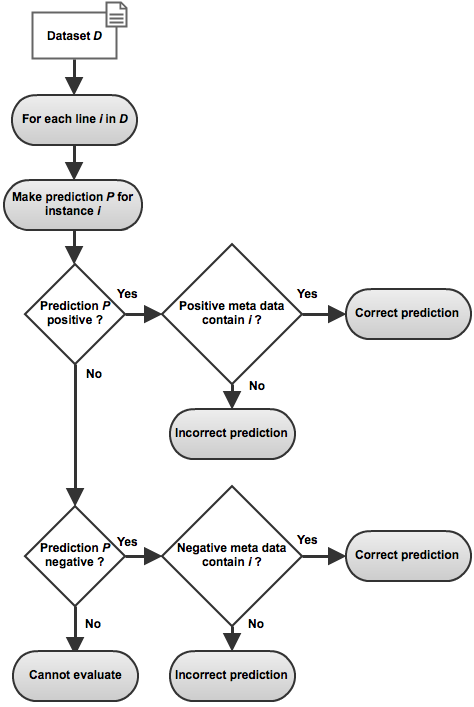
\includegraphics[keepaspectratio,scale=0.464]{MetaDataEvalFlow.png}
    \else
      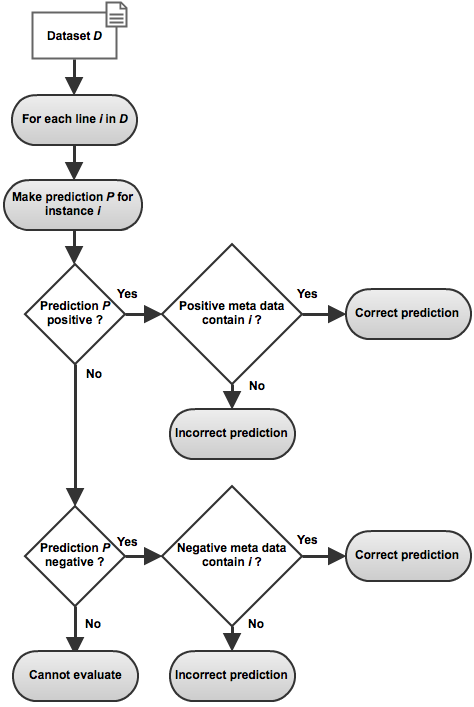
\includegraphics[keepaspectratio,scale=0.464]{MetaDataEvalFlow.png}
    \fi
    \caption[An overview of how meta data is used during evaluation.]{An overview of how meta data is used during evaluation.}
    \label{metadata}
  \end{center}
\end{figure}
\newpage
\subsubsection{Meta data for Sampling}
Meta data plays an important role in the sampling of data sets. During the sampling of two class binary data set $D$, the positive and negative ARFF meta data files (described above), are used to create a hash map based data structure similar to that used during evaluation. The hash maps for the positive and negative classes respectively, can be used to randomly select instances in $D$. This actually corresponds to selecting line numbers in $D$. Therefore to randomly select instances to include in a sampling, all we need to do is randomly select line numbers from these hash maps. This allows a sampling to be created even when the data set has only been read once. Lets extending the example used in the previous section. To sample positive examples, all we need to do is simply choose a random number between 1-3 (the key value).

\begin{figure}[!htbp]
  \begin{center}
    \leavevmode
    \ifpdf
      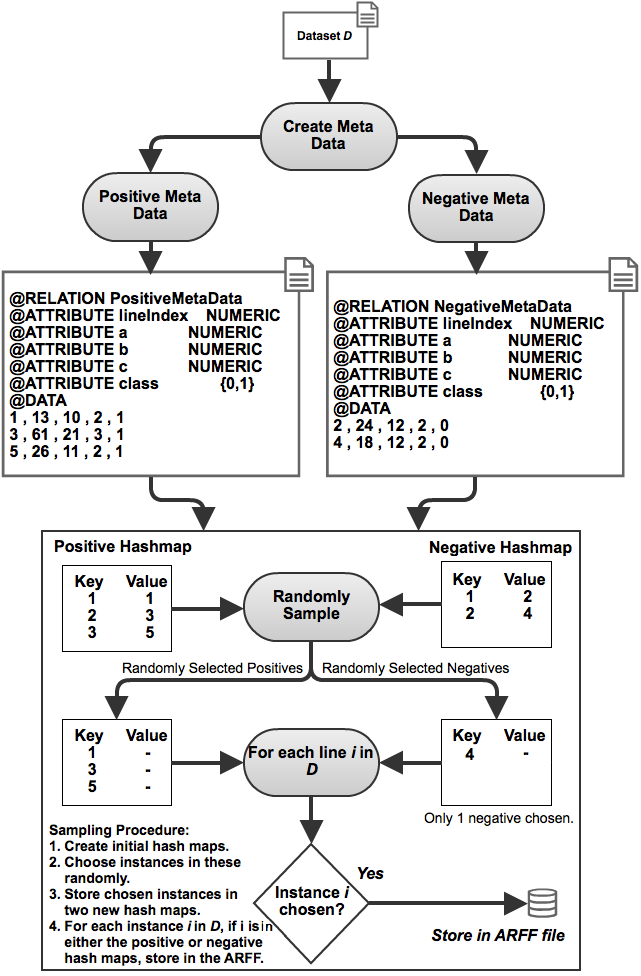
\includegraphics[keepaspectratio,scale=0.45]{MetaData.png}
    \else
      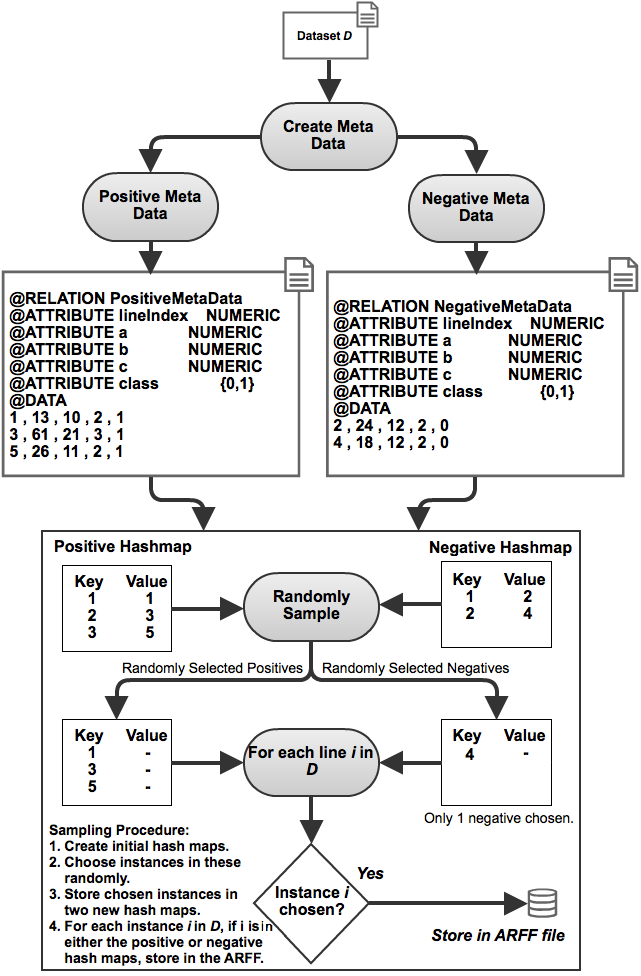
\includegraphics[keepaspectratio,scale=0.45]{MetaData.png}
    \fi
    \caption[An overview of the meta data creation procedure, and the role of meta data in sampling data sets.]{An overview of the meta data creation procedure, and the role of meta data in sampling data sets.}
    \label{metadataroleinsampling}
  \end{center}
\end{figure}
Training and test sets are built in this manner, by randomly sampling from these hash maps. In other words, given a specified training set size and class distribution, the required number of random samplings can be made from these hash maps. To then create a training set, the original file $D$ is read for a second time. On this second pass, when a line number corresponding to a randomly chosen positive or negative is encountered, it is written to a separate training set file. Test sets are constructed similarly, except that examples chosen for the training set, cannot occur in the test set. As the sampling procedure used is random, training and test sets vary with each sampling run.

This approach is by no means optimal, although it appears to work well in practice. However there are some clear drawbacks. Firstly, the larger the dataset, the longer it will take to produce a larger test/train sample. Whilst this may seem obvious, it is certainly worth emphasising before embarking upon sampling a file with millions of instances. In practice, the amount of time taken to sample a dataset containing 10 million instances, will take anywhere between 10-20 minutes - assuming a standard disk. The precise time depends entirely on the I/O speed of the hard disk used, and the operating system load at sample time\footnote{On a solid state drive, this takes only 1 or 2 minutes.}. In general the amount of time it takes to sample a dataset $D$, scales with the number of instances to be included in the sample. Secondly, the completion time of this approach is effected by how many times a random number generator chooses a line index, previously selected. As a uniform random number generator is used, the same index is likely to be chosen multiple times, thus increasing the runtime, as a new random index must then be generated.

\subsection{Sampling}
\label{sec:sampling}
\textsc{stuffed} may be required to create new training/test data streams from very large binary datasets. Here we consider a very large dataset to be one infeasible to load into memory. In practice any data set which is more than a few gigabytes in size, is difficult to load into memory, especially given that an internal representation of the file usually requires more memory than the file footprint. Thus, any sampling procedure must be able to sample these files without loading them into memory, and preferably in a single pass. This is not a hugely complex task, but it is comprised of many steps. We present the sampling algorithm here in full to facilitate an understanding of the code, and explain precisely how this particular procedure works. We begin by explaining the mathematical foundation of the sampling procedure, before presenting the sampling algorithm.\\
\subsubsection{Sampling Foundation}
To sample a data set $D$, we need to know what the desired test/training sets should look like. There are many possible configurations for these datasets. Let us assume that we firstly wish to alter the class balance, in both the training and test sets. Each dataset $D$ has a natural balance $b$, which we may wish to alter. The class balance for the training set $D_{train}$ is given by,
\begin{eqnarray*}
D_{train}^{b}=\frac{\textrm{positives in training set}}{\textrm{negatives in training set}} \textrm{,}
\end{eqnarray*}
and is defined as the ratio between the positive and negative classes. Likewise for the test set $D_{test}$, the balance $D_{test}^{b}$ is defined similarly. To change these balances we must specify a new class balance ratio. We must then populate $D_{train}$ and $D_{test}$ with instances from $D$, ensuring that the ratios $D_{train}^{b}$ and $D_{test}^{b}$ are adhered to. 

However it may not be possible to satisfy a desired training/test set balance, for a given data set $D$. For instance if $D$ contains $1000$ instances, of which there are +500 : -500, then a test data set with a +1 : -1000 balance simply cannot be created. This raises the question of how many examples would be required to achieve that level of imbalance? We can answer this question with some basic mathematics. To make such a test set, we require a number of negative test set instances given by,

\begin{eqnarray*}
D_{test}^{-}=\frac{D_{test}^{+}}{D_{test}^{b}}\textrm{,}
\end{eqnarray*} 
where $D_{test}^{-}$ is the number of negatives in the test set, $D_{test}^{+}$ the number of positives in the test set, and $D_{test}^{b}$ the desired balance. Thus we require in this example,

\begin{eqnarray*}
\frac{1}{0.001}=1000\textrm{,}
\end{eqnarray*}

negative instances. Clearly there are not enough negatives to satisfy the desired balance, so this sampling cannot be achieved.

\begin{table}[htp]
\centering
    \begin{tabular}{|l|l|}
    \hline
    Variable & Description \\ \hline
    $D$        & The input data set.           \\[1ex]
    $D^{+}$        & The number of positives in the data set $D$.           \\[1ex]
    $D^{-}$        & The number of negatives in the data set $D$.           \\[1ex]
    $D_{tot}$        & The number of positives and negatives in the data set $D$.           \\[1ex]
    $D_{train}^{+}$        & Positives in the training set.           \\[1ex]
    $D_{train}^{-}$        & Negatives in the training set.           \\[1ex]
    $D_{train}^{max}$        & Maximum number of instances allowed in the training set.           \\[1ex]
    $D_{train}^{b}$        & Training set class balance.           \\[1ex]
    $D_{test}^{+}$        & Positives in the test set.           \\[1ex]
    $D_{test}^{-}$        & Negatives in the test set.           \\[1ex]
    $D_{test}^{max}$        & Maximum number of instances allowed in the test set.           \\[1ex]
    $D_{test}^{b}$        & Test set class balance.           \\[1ex]
    $skipablePositives$        & The number of positives that can be left out.           \\[1ex]
    $skipableNegatives$        &  The number of negatives that can be left out.          \\[1ex]
    $D_{test}^{l}$                   & The ratio of labelled instances in the test set. \\[1ex]
    $F$                   & The features to use. \\\hline
    \end{tabular}
    \caption[The primary variables used for data set sampling.]{The variables used for data set sampling.}
\label{tab:vars}
\end{table}

The previous example does not consider what happens when a training set must also be created. Creating a training set only slightly complicates matters. 

Let us imagine that we have a data set $D$ with $1500$ instances, of which there are $D^{-}=1000$ negatives and $D^{+}=500$ positives. The goal is to sample this data set to produce a training set with 50 positives, $D_{train}^{+}=50$, with a balance $D_{train}^{b}=\frac{1}{2}=0.5$, and a test set with a balance of $D_{test}^{b}=\frac{2}{5}=0.4$. 

Firstly we must find the parameters of the training set. The number of negatives in the training set is given by,
\begin{eqnarray*}
D_{train}^{-}=D_{train}^{+} \div D_{train}^{b}\textrm{.}
\end{eqnarray*}
Upon substituting in our values gives,
\begin{eqnarray*}
D_{train}^{-}=50\div 0.5=100\textrm{.}
\end{eqnarray*}
Now we try to find the parameters for the test set. The number of positives in the test set is given by,
\begin{eqnarray*}
D_{test}{+}=D^{+}-D_{train}^{+}\textrm{.}
\end{eqnarray*}
This gives us $D_{test}{+}=450$. The number of negatives required in the test set then is given by,
\begin{eqnarray*}
D_{test}^{-}=D_{test}^{+}\div D_{test}^{b}\textrm{,}
\end{eqnarray*}
which is $D_{test}^{-}=450 \div 0.4 = 1125$. As $D_{test}^{-} < (D^{-}-D_{train}^{-})$ (enough negatives left over after creating the training set) then clearly this is an ideal situation in which everything works well. In situations where,
\begin{eqnarray*}
D_{test}^{-} > (D^{-}-D_{train}^{-})\textrm{,}
\end{eqnarray*}
then we must modify the parameters. In particular we reset,
\begin{eqnarray*}
D_{test}^{-}=D^{-}-D_{train}^{-}\textrm{,}
\end{eqnarray*}
and then obtain,
\begin{eqnarray*} 
D_{test}^{+}=D_{test}^{-}\times D_{test}^{b}\textrm{.}
\end{eqnarray*} 
The variables introduced are listed in Table \ref{tab:vars}. Those we have not described so far are $skipablePositives$ and $skipableNegatives$, which are simply counts of the number of positive and negative instances respectively that will be not used in the sampling (i.e. left over instances). Whilst $F={ \lbrace (f_{i}),...,(f_{n})\rbrace}$, $i=1,...,n$ where $f_{i} \in \mathbb{Z} $ is the array of features to use.

Aside from the ability to rebalance a dataset, the requirements for the sampling procedure set out in section \ref{sec:requirements}, also describe the need to vary the labelling of the test data $D_{test}$. The variable $D_{test}^{l}$ introduced in Table \ref{tab:vars} helps to achieve this, irrespective of the balance of $D_{test}$. The variable $D_{test}^{l}$ is defined as, 
\begin{eqnarray*}
D_{test}^{l}=\frac{\textrm{ Labelled instances in } D_{test}}{\textrm{ total instances in } D_{test}} \textrm{.}
\end{eqnarray*}
Thus by determining a value for $D_{test}^{l}$, we can ensure a test data set contains the desired ratio of labelled to unlabelled instances, by simply keeping track of those instances labelled.
\newpage
\subsubsection{Sampling Algorithm}
With the principal variables defined we now begin to present the psuedocode for the algorithmic sampling procedure.
\begin{algorithm}
\small
\caption{Part 1: Variable Initialisation}
\begin{algorithmic}[1]
\Require An input dataset $D$, a destination training set file path $trainPath$, a destination test set file path $testPath$, the number of positive training samples $D_{train}^{+}$, the desired training set balance $D_{train}^{b}$, the desired test set balance $D_{test}^{b}$, the labelling ratio $D_{test}^{l}$, and an array of features to use $F$.
%\Ensure A test dataset $D_{test}$ and a training set $D_{train}$.
\Procedure {sample}{$D$, $out$, $D_{train}^{+}$, $D_{train}^{b}$,$D_{test}^{b}$,$l$,$F$}
\State $classDist[] \leftarrow$ getClassDistribution()
\State $D^{-} \leftarrow classDist[0]$ 
\State $D^{+} \leftarrow classDist[1]$
\State $D_{tot} \leftarrow D^{+}+D^{-}$ 
\State $D_{train}^{-} \leftarrow D_{train}^{+} \div D_{train}^{b}$
\State $D_{train}^{max} \leftarrow D_{train}^{-}+D_{train}^{+}$
\State $D_{test}^{+} \leftarrow D^{+}-D_{train}^{+}$ 
\State $D_{test}^{-} \leftarrow D_{test}^{+} \div D_{test}^{b}$
\If {$D_{test}^{-} > (D^{-}-D_{train}^{-})$}
	\State $D_{test}^{-}  \leftarrow D^{-}-D_{train}^{-}$
	\State $D_{test}^{+}  \leftarrow D_{test}^{-} \times D_{test}^{b}$
\EndIf
\State $D_{test}^{max} \leftarrow D_{test}^{+}+D_{test}^{-}$
\State $skipablePositives \leftarrow (D^{+}-D_{train}^{+})-D_{test}^{+}$
\State $skipableNegatives \leftarrow (D^{-}-D_{train}^{-})-D_{test}^{-}$
               \State \Comment continued in Part 2...
\algstore{bkbreak}
\end{algorithmic}
\end{algorithm}

The code in part 1 sets up the key parameter variables necessary to perform the sampling. The call to $getClassDistribution()$ in step 2 simply returns an array with two components, where component zero contains the number of negative instances in $D$, while component one contains the number of positives. At this stage we now know exactly how many positive and negative instances we require in the training/test data sets, and what proportion of the data should be labelled. To actually perform the sampling then we must read in each instance $x_{i}$ from $D$ one at a time, and decide what to do with it. There are three distinct possibilities,
\begin{enumerate}
 \item Insert instance $x_{i}$ in to the training set.
 \item Insert instance $x_{i}$ in to the test set and label it.
 \item Insert instance $x_{i}$ in to the test set and remove its label.
 \end{enumerate} 
In order to decide what to do, we randomly select instances to insert in to the test and training sets, using meta data described in Section \ref{sec:stfuddata}.  There are some further variables which must be initialised before this can be achieved. This is because in order to sample the data set in a single pass \footnote{Strictly speaking the sampling is not single pass, as meta data must be obtained before hand.}, we must keep a count of,
\begin{enumerate}
\item those instances which have been inserted in to the positive and negative training sets.
\item how many of those were labelled.
\item which particular instance $x_{i}$ in $D$ we are up to.
\end{enumerate}
\newpage
These extra variables are summarised in Table \ref{tab:vars2} below.

\begin{table}[htp]
\centering
    \begin{tabular}{|l|l|}
    \hline
    Variable & Description \\ \hline
    $toLabel$        & The number of instances in $D_{test}$ to label.           \\[2ex]
    $notToLabel$        & The number of instances in $D_{test}$ not to label.            \\[2ex]
    $labelled$        & A count of the instances labelled in $D_{test}$.           \\[2ex]
    $unlabelled$        & A count of the instances unlabelled in $D_{test}$.           \\[2ex]
    $negInTrainingSet$        & A count of the negatives put in the training set.           \\[2ex]
    $negInTestSet$        & A count of the negatives put in the test set.           \\[2ex]
    $posInTrainingSet$        & A count of the positives put in the training set.           \\[2ex]
    $posInTestSet$        & A count of the positives put in the test set.           \\[2ex]
    $trainingSetCount$        & A count of the instances put in the training set.           \\[2ex]
    $testSetCount$        & A count of the instances put in the test set.           \\[2ex]
    $instanceIndex$        & The current index $i$ of the instance $x$.           \\\hline
    \end{tabular}
    \caption[The secondary variables used for data set sampling.]{The secondary variables used for data set sampling.}
\label{tab:vars2}
\end{table}
With these additional variables described, we move on to consider the remainder of the algorithm. There are two components worthy of note. The first randomly selects candidates to include in the sample, using the meta data described in Section \ref{sec:stfuddata}. Meta data are stored in a hash map based data structure on lines 31-32 of algorithm 2, one hash map per class. The key for these data structures is simply an integer representing the order an instance was inserted into the map, whilst the value contains the line each instance can be found at in $D$. For the positive class, this data structure can be described abstractly by the following table.
\begin{table}[!htp]
\centering
\footnotesize
    \begin{tabular}{|l|l|}
    \hline
    Key & Value \\ \hline
    $<$Instance 1$>$ & $<$Instance line number in $D>$  \\
    $<$Instance 2$>$ & $<$Instance line number in $D>$  \\
    ... & ... \\
    $<$Instance $D^{+}-1>$ & $<$Instance line number in $D>$ \\
    $<$Instance $D^{+}>$ & $<$Instance line number in $D>$ \\\hline
    \end{tabular}
     \caption[An example of the positive hash data structure.]{An example of the positive hash data structure.}
     \label{tab:hashmapabstract}
\end{table}
\newpage
A random number generator is used to choose instances to use. The generator chooses values in the range $[1,N]$, where N is the total number of instances in the hash map. In the case of the positive hash map described in Table \ref{tab:hashmapabstract}, the range would be  $[1,D^{+}]$.
\begin{algorithm}[!h]
\small
\caption{Part 2}
\begin{algorithmic}[1]
\algrestore{bkbreak}
\State toLabel $\leftarrow (D_{test}^{+}+D_{test}^{-}) \times D_{test}^{l}$
\State notToLabel $\leftarrow (D_{test}^{+}+D_{test}^{-}) - toLabel$
\State labelled $\leftarrow 1$
\State unlabelled $\leftarrow 1$
\State negInTrainingSet$\leftarrow 0$
\State negInTestSet$\leftarrow 0$
\State posInTrainingSet$\leftarrow 0$
\State posInTestSet$\leftarrow 0$
\State testSetCount$\leftarrow 0$
\State trainingSetCount$\leftarrow 0$
\State instanceIndex$\leftarrow 0$
\State writeCounter $\leftarrow 0$
\State testSetString$\leftarrow$ null
\State HashMap$<$int,int$>$ $positives \leftarrow getMetaData(pathToPositiveMetaData)$
\State HashMap$<$int,int$>$ $negatives \leftarrow getMetaData(pathToNegativeMetaData)$
\State posTrainingSet $\leftarrow HashMap<int,bool>$
\State posTestSet $\leftarrow HashMap<int,bool>$
\State negTrainingSet $\leftarrow HashMap<int,bool>$
\State negTestSet $\leftarrow HashMap<int,bool>$
\State $r \leftarrow new$ $Random()$
\State \Comment continued in Part 3...
\algstore{bkbreak}
\end{algorithmic}
\end{algorithm}

It is then simply a case of populating the hash maps declared in lines 33-36 of algorithm 2, with those instances randomly selected. The pseudocode for how this is achieved is presented below. For brevity we only show the code applicable for selecting positive instances for the training set.
\begin{algorithm}[!h]
\small
\caption{Part 3}
\begin{algorithmic}[1]
\algrestore{bkbreak}
\While{ $(posTrainingSet.size() < D_{train}^{+} )$}
	\State $randIndex \leftarrow r.nextInt(0,D^{+})$
			\If{$(positives.get(randIndex) \neq null)$}
				\While{$(posTrainingSet.hasKey(positives.get(randIndex)))$}
					\State $randIndex \leftarrow r.nextInt(0,D^{+})$
				\EndWhile
			\EndIf
			\State $posTrainingSet.put(positives.get(randIndex), true);$
\EndWhile
\State \Comment continued in Part 4...
\algstore{bkbreak}
\end{algorithmic}
\end{algorithm}

In the code above $nextInt()$ is a method that returns a random number uniformly distributed in a range specified, using minimum and maximum values. The $get(int)$ method on the other hand, simply returns a value from the hash map specified by the supplied integer key.

Once the instances to be used in the sampling have been selected, the next crucial component reads the data file $D$, and writes each candidate to either i) a destination training set, ii) a destination test set, or iii) neither if not selected. The final part of the sampling procedure that makes these determinations, is presented overleaf.
\newpage
The while loop on line 50 simply iterates over the dataset $D$, until both the training and test data are filled with instances. The calls to $Write()$ simply write out the current instance to the specified file. On line 64 and 74, the $label()$ function is used to decided whether or note a instance should be labelled. The pseudocode for this procedure is also presented for completeness overleaf.
\begin{algorithm}[!h]
\small
\caption{Part 4}
\begin{algorithmic}[1]
\algrestore{bkbreak}
\State $i \leftarrow 0$
   \While{$(i < D_{tot} \land (trainingSetCount < D_{train}^{max}) \land (testSetCount < D_{test}^{max}) )$}
      \State $i\gets i+1$
      \State $Instance \leftarrow D.readLine()$
      \If {$(posTrainingSet.containsKey(i))$}
      	\State $posInTrainingSet \gets posInTrainingSet+1$
      	\State $trainingSetCount \gets trainingSetCount+1$
      	\State $Write(trainPath,Instance)$
      \ElsIf{$(negTrainingSet.containsKey(i))$}
      \State $negInTrainingSet \gets negInTrainingSet+1$
      	\State $trainingSetCount \gets trainingSetCount+1$
      	\State $Write(trainPath,Instance)$
      	\ElsIf{$(posTestSet.containsKey(i))$}
      \State $posInTestSet \gets posInTestSet+1$
      	\State $testSetCount \gets testSetCount+1$
      	\If{ $label(labelled,unlabelled,toLabel,notToLabel,D_{test}^{l})$}
      		\State $labelled \leftarrow labelled +1$
      		\State $Write(testPath,Instance)$
      	\Else
      	\State $unlabelled \leftarrow unlabelled +1$
      		\State $Write(testPath,RemoveLabel(Instance))$
      	\EndIf
      	 \Else{$(negTestSet.containsKey(i))$}
      \State $negInTestSet \gets negInTestSet+1$
      	\State $testSetCount \gets testSetCount+1$
      	\If{ $label(labelled,unlabelled,toLabel,notToLabel,D_{test}^{l})$}
      		\State $labelled \leftarrow labelled +1$
      		\State $Write(testPath,Instance)$
      	\Else
      	\State $unlabelled \leftarrow unlabelled +1$
      		\State $Write(testPath,RemoveLabel(Instance))$
      	\EndIf
      \EndIf
   \EndWhile
\EndProcedure
\end{algorithmic}
\end{algorithm}
\clearpage
Here is the labelling procedure:
\begin{algorithm}[!h]
\small
\caption{Labelling Procedure}
\begin{algorithmic}[1]
\Require The number of instances currently with labels $labelled$, the number of instances not labelled $unlabelled$, the number of instances that must be labelled $toLabel$, the number of instances that must not be labelled $notToLabel$, and the labelling ratio $D_{test}^{l}$.
\Ensure True if an item should be labelled, else false.
\Procedure {label}{$labelled$, $unlabelled$, $toLabel$, $notToLabel$,$D_{test}^{l}$}
\State $r \leftarrow new$ $Random()$
\State $result \leftarrow 0$
\While{ $(result = 0)$}
	\State $rand \leftarrow r.nextDouble()$
	\State $result \leftarrow compare(rand,D_{test}^{l})$
\EndWhile
\If{$(compare(D_{test}^{l},1)=0)$} \Comment $D_{test}^{l}=1$ label every instance.
	\State \Return true
\ElsIf{$(compare(D_{test}^{l} ,0.0)=0)$} \Comment $D_{test}^{l}=0$ label none.
	\State \Return false
\Else
	\If{$(result >0 \land (unlabelled < notToLabel))$}
	\State \Return false
	\ElsIf{$(result <0 \land (labelled < toLabel))$}
	\State \Return true
	\ElsIf{$(result >0 \land (unlabelled < notToLabel))$}
	\State \Return true
	\Else
		\State \Return false
	\EndIf
\EndIf
\EndProcedure
\end{algorithmic}
\end{algorithm}

This procedure decides if an instance should be labelled, by first choosing a random number $rand$, in the interval $[0,1]$. If $rand < D_{test}^{l}$, then the instance will be labelled. Else it will not be labelled. For instance, if $D_{test}^{l}=0.75$ (i.e. 75\% of the instances should be labelled), then $0 < rand < 0.75$ will result in the instance being labelled, and if $ 0.75 < rand < 1$ it will not be labelled. Here the call to $nextDouble()$, returns a random double value generated uniformly in the interval $[0,1]$. Whilst $compare(a,b)$, returns zero if $a = b$, a value less than zero when $a < b$, else a value greater than 0 is returned. 
\newpage
\subsection{Evaluation}
\label{sec:evaluation}
The procedure which \textsc{stuffed} uses to execute and evaluate tests, is summarised in Figure \ref{fig:framework}. A discrete time model is adopted for each classifier test, thus per instance $x_{i}$ arriving at time step $t$, a class prediction is made at time step $t+1$. The classifier model is then updated via training at time step $t+2$, but only if the instance was labelled in the stream. This corresponds to an incremental, rather than a batch processing approach to learning \footnote{In the batch processing scenario, at time $t$ a batch $b$ of $n$ unlabelled instances would be received and classified using a model trained on batches $b_{1}$ to $b_{t-1}$. At time $t+1$ labels arrive for batch $b_{t}$, along with a new batch of unlabelled instances $b_{t+1}$.}.

\begin{figure}[htb]
	\centering
		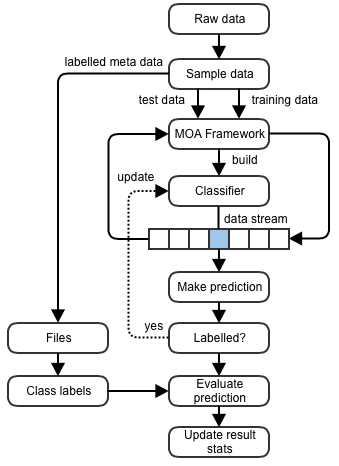
\includegraphics[keepaspectratio,scale=0.6]{Framework.png}
		\caption[An overview of the test and evaluation procedure.]{An overview of the test test and evaluation procedure.}
		\label{fig:framework}
		\vspace{-1em}
\end{figure}

Following each prediction a count of true positives (TP), false positives (FP), false negatives (FN) and true negatives (TN) is updated, by checking the prediction against the correct label of $x_{i}$. If $x_{i}$ was unlabelled in the stream, then the correct label is obtained from a meta data file, and compared to the prediction as before. Thus each prediction is evaluated during testing. However, overall evaluation statistics are not computed until the end of a test run.

This incremental evaluation differs slightly, from the two most common approaches used for evaluating classifier performance under the batch paradigm. The first of these evaluates classifier performance on a single batch of data, selected from among the many batches in the stream. The batch selected is usually the last one received from the stream, on the assumption that performance on the last batch is representative of performance on the stream as a  whole. 

The second evaluates performance over all the batches in the stream using some measure of average performance. The former approach is unsuitable for evaluating classifier performance in our problem domain, as evaluating a single batch from an imbalanced stream, can be extremely misleading. Consider the following illustrative example. Suppose we have a stream containing 1 million instances, imbalanced such that there are 10,000 negative examples for each positive. Even with a batch size as large as 10,000 instances, given that positives occur randomly and infrequently in the stream, it is possible that any arbitrary batch chosen for evaluation will contain zero positive instances. Such a batch says little about classifier performance on the minority positive class. In terms of evaluating across all batches using some averaging metric, whilst this approach is preferable to evaluating on a single batch, it is not without problems. For imbalanced streams such averages will also provide a misleading impression of performance, given that most measures of accuracy will tend towards one, as more batches from the stream are seen (see discussion below). In practice the incremental evaluation approach employed by \textsc{stuffed}, has greater precision given that absolute statistics rather than averages, are maintained throughout.

Any evaluation performed on the streams described thus far, must account for class imbalance. However evaluating classifier performance on imbalanced data is known to be difficult, particularly as many metrics are sensitive to the underlying class distribution \cite{Haibo:2009:fb}. Using these metrics can provide misleading, often positive impressions of performance. One such metric to which this happens is classifier accuracy (see Eq. \ref{eq:accuracy}). Accuracy is acutely effected by class imbalance, and this can be illustrated using a simple example. Suppose we have a stream of data imbalanced in favour of the negative class. A hypothetical classifier which is 100\% accurate on the negative class and 0\% accurate on the positive class, has an accuracy that tends towards 1, as the number of instances classified $n=TN+TP+FP+FN$ becomes larger,\\
\begin{eqnarray} \label{eq:limi1}
\lim_{TN\to \infty} \frac{TP+TN}{TP+TN+FP+FN} = 1 \textrm{ ,}
\end{eqnarray}\\
where $TP$ is the number of instances correctly classified as positive (in this case zero), and $TN$ the number of instances correctly classified as negative. If actively monitoring classifier accuracy, we must then be prepared for misleading results. In any case, a single metric will tell us little with regards to classifier performance. Therefore \textsc{stuffed} keeps track of multiple assessment metrics. Some of these are described in Table \ref{tab:metrics}. 
\newpage
These include amongst others the F-Score and the G-Mean \cite{Haibo:2009:fb}. The F-Score is monitored due to its widespread use by the machine learning community, however we note that the F-Score is sensitive to changes in the class distribution, given its dependence on precision. Thus when a data set is large and imbalanced, the numerator of the F-Score equation remains small, while the denominator becomes increasingly large. Thus low precision can cause the F-Score to obtain a small value, even given a high level of recall. The G-Mean however is not sensitive to the class distribution in the same way. It evaluates the inductive bias in terms of the ratio between positive and negative accuracy. Together then these two metrics give a representative view of classifier performance which should allow a comparison between algorithms tested within \textsc{stuffed} and other data mining tools.
\begin{table}
\small
\centering
\begin{tabular}{|m{1.2cm}|m{3cm}|c|}
\hline
{\bf Statistic} & {\bf Description} & {\bf Definition} \\ 
\hline\hline	
Accuracy & Overall accuracy. & $\frac{(TP+TN)}{(TP+FP+FN+TN)}$ \\
\hline
False positive rate (FPR) & Fraction of negative instances incorrectly labelled positive. & $\frac{FP}{(FP +TN)}$\\
\hline
F-Score & Measure of accuracy that considers both precision and recall. & $2\times{ \frac{precision\times{recall}} {precision + recall}} $\\
\hline
G-Mean & Imbalanced data metric describing the ratio between positive and negative accuracy. & $\sqrt{\frac{TP}{TP+FN}\times \frac{TN}{TN+FP}}$\\
\hline	
Precision & Fraction of retrieved instances that are positive. & $\frac{TP}{(TP+FP)}$ \\
\hline
Recall & Fraction of positive instances that are retrieved. & $\frac{TP}{(TP + FN)}$\\
\hline	
Specificity & Fraction of negatives correctly identified as such. & $ \frac{TN}{(FP + TN)}$ \\
\hline
\end{tabular}
\caption[Standard evaluation metrics for classifier performance.]{Standard evaluation metrics for classifier performance. True Positives (TP), are those candidates correctly classified as pulsars. True Negatives (TN) are those correctly classified as \textit{not} pulsars. False Positives (FP) are those incorrectly classified as pulsars, finally False Negatives (FN) are those incorrectly classified as \textit{not} pulsars. All metrics produce values in the range $[0,1]$. }
 \label{tab:metrics}
 \vspace{-1.0em}
\end{table}

\newpage
\bibliography{References.bib}
\bibliographystyle{ieeetr}

\printindex

\end{document}